\documentclass{article}
\usepackage[T2A]{fontenc}
\usepackage[utf8]{inputenc}
\usepackage[english,russian]{babel}
\usepackage{amsmath}
\usepackage{amssymb}
\usepackage{geometry}
\geometry{a4paper,scale=0.7}
\usepackage{graphicx}
\usepackage{listings}
\usepackage{pythonhighlight}
\usepackage{algorithm}
\usepackage{algorithmic}
\usepackage{makecell}
% first row with two sapce 
\usepackage{indentfirst}
\setlength{\parindent}{2em}
\usepackage{hyperref}
\hypersetup{
	colorlinks=true,
	linkcolor=black
}

\usepackage{listings}

\usepackage{xcolor}

%New colors defined below
\definecolor{codegreen}{rgb}{0,0.6,0}
\definecolor{codegray}{rgb}{0.5,0.5,0.5}
\definecolor{codepurple}{rgb}{0.58,0,0.82}
\definecolor{backcolour}{rgb}{0.95,0.95,0.92}

%Code listing style named "mystyle"
\lstdefinestyle{mystyle}{
  backgroundcolor=\color{backcolour}, commentstyle=\color{codegreen},
  keywordstyle=\color{magenta},
  numberstyle=\tiny\color{codegray},
  stringstyle=\color{codepurple},
  basicstyle=\ttfamily\footnotesize,
  breakatwhitespace=false,         
  breaklines=true,                 
  captionpos=b,                    
  keepspaces=true,                 
  numbers=left,                    
  numbersep=5pt,                  
  showspaces=false,                
  showstringspaces=false,
  showtabs=false,                  
  tabsize=2
}

%"mystyle" code listing set
\lstset{style=mystyle}

\title{Отчет по дополнительному заданию курса \\
“Суперкомпьютерное моделирование и технологии”\\
Численное решение задачи математической физики \\
с использованием технологий MPI+OpenACC}
\author{Сюй Минчуань, группа 617, номер варианта: 8}
\date{\today}

\begin{document}
\maketitle
\tableofcontents

\newpage
\section{Постановка задачи}

Предлагается решить задачу краевую задачу для уравнения Пуассона с потенциалом в прямоугольной области методом конечных разностей.

Рассматривается в прямоугольнике $\Pi = \{(x,y): A_1 \leqslant x \leqslant A_2, B_1 \leqslant y \leqslant B_2\}$ дифференциальное уравнение Пуассона с потециалом
\begin{equation*}
    -\Delta u + q(x,y)u = F(x,y)
\end{equation*}
в котором оператор Лапласа 
\begin{equation*}
    \Delta u = \frac{\partial}{\partial x} \left(k(x,y)\frac{\partial u}{\partial x} \right) + \frac{\partial}{\partial y}\left(k(x,y)\frac{\partial u}{\partial y} \right)
\end{equation*}

В частности, для \textbf{варианта 8} нужно восстановить функцию $u(x,y)=\sqrt{4+xy}, \Pi = [0,4] \times [0,3]$ с коэффциентом $k(x,y) = 4 + x + y$ и потенциалом $q(x,y) = x + y$. 

Для выделения единственного рещения уравнения понадобятся граничные условия. В своём варианте для левой ($\gamma_L$) и правой ($\gamma_R$) границы задано условие третьего типа:
\begin{equation*}
    \left( k\frac{\partial u}{\partial n}\right)(x,y) + u(x,y) = \psi(x,y)
\end{equation*}
а для верхней ($\gamma_T$) и нижней ($\gamma_B$) границы задано условие второго типа:
\begin{equation*}
    \left( k\frac{\partial u}{\partial n}\right)(x,y) = \psi(x,y)
\end{equation*}
где $n$ - единичная внешняя нормаль к границе. Так как в угловых точках области нормаль не определена, то краевое условие рассматривается лишь в тех точках границы, где есть нормаль.

Необходимо определить правую часть $F(x,y)$, сначала вычислить $-\Delta u$:
\begin{equation*}
\begin{aligned}
    - \Delta u &= - \frac{\partial}{\partial x} \left((4+x+y)\frac{\partial}{\partial x}\sqrt{4+xy} \right) - \frac{\partial}{\partial y}\left((4+x+y)\frac{\partial}{\partial y}\sqrt{4+xy} \right) \\
    &= - \frac{\partial}{\partial x} \left(\frac{y(4+x+y)}{2\sqrt{4+xy}}\right) - \frac{\partial}{\partial y} \left(\frac{x(4+x+y)}{2\sqrt{4+xy}}\right) \\
    &= - \frac{y\cdot 2\sqrt{4+xy}-y^2(4+x+y)(\sqrt{4+xy})^{-1}}{4(4+xy)} - \frac{x\cdot 2\sqrt{4+xy}-x^2(4+x+y)(\sqrt{4+xy})^{-1}}{4(4+xy)} \\
    &= \frac{(4+x+y)(x^2+y^2)-2(x+y)(4+xy)}{4(4+xy)^{3/2}}
\end{aligned}
\end{equation*}
Значит
\begin{equation*}
    F(x,y) = \frac{(4+x+y)(x^2+y^2)-2(x+y)(4+xy)}{4(4+xy)^{3/2}} + (x+y)\sqrt{4+xy}
\end{equation*}
а ещё граничные условия:
\begin{equation*}
\begin{aligned}
    &\gamma_L: \psi_L(x,y) = (4+x+y)\cdot\left(\frac{-y}{2\sqrt{4+xy}}\right) + \sqrt{4+xy} = \{ \text{при } x=0\} = \frac{1}{4}\cdot(8-4y-y^2)\\
    &\gamma_R: \psi_R(x,y) = (4+x+y)\cdot\left(\frac{y}{2\sqrt{4+xy}}\right) + \sqrt{4+xy} = \{ \text{при } x=4\} = \frac{y^2+16y+8}{4\sqrt{1+y}}\\
    &\gamma_T: \psi_T(x,y) = (4+x+y)\cdot\left(\frac{x}{2\sqrt{4+xy}}\right) = \{ \text{при } y=3\} = \frac{x(7+x)\sqrt{4+3x}}{2(4+3x)}\\
    &\gamma_B: \psi_B(x,y) = (4+x+y)\cdot\left(\frac{-x}{2\sqrt{4+xy}}\right) = \{ \text{при } y=0\} = -\frac{1}{4}(x^2+4x)\\
\end{aligned}
\end{equation*}


\section{Численный метод решения}
\subsection{Разностная схема решения задачи}

Предлагается методом конечных разностей решить данную задачу. В рассматриваемой области $\Pi$ определяется равномерная сетка $\bar{\omega_h} = \bar{\omega_1} \times \bar{\omega_2}$, где
\begin{equation*}
    \bar{\omega_1} = \{x_i = A_1 + ih_1, i=\overline{0,M} \}, \bar{\omega_2} = \{y_j= B_1 + jh_2, j=\overline{0,N} \}
\end{equation*}
здесь $h_1 = (A_2 - A_1)/M, h_2 = (B_2-B_1)/N$. Рассмотрим линейное пространство $H$ функций, заданных на сетке $\bar{\omega_h}$. Обозначим через $\omega_{ij}$ значение сеточной функции $\omega\in H$ в узле сетки $(x_i, y_i)$. Будем считать, что в пространстве $H$ задано скалярное произведение и норма
\begin{equation*}
    [u,v] = \sum_{i=0}^{M} h_1 \sum_{j=0}^{N} h_2\rho_{ij}u_{ij}v_{ij}, \quad \|u\|_E = \sqrt{[u,u]}
\end{equation*}
где весовая функция $\rho_{ij}$ равна $1$ когда $\omega_{ij}$ - внутренний узел; равна $1/2$ когда граничный узел и равна $1/4$ когда угловый узел. Уравнение во всех внутренних точках сетки аппроксимируется разностным уравнением
\begin{equation*}
    -\Delta_h \omega_{ij} + q_{ij}\omega_{ij} = F_{ij}, \quad i=\overline{1,M-1}, j=\overline{1,N-1}
\end{equation*}
в котором $F_{ij} = F(x_i, y_j), q_{ij} = q(x_i, y_j)$, а разностный оператор Лапласа $-\Delta_{h}\omega_{ij}$ можно записать в виде $\Delta_h\omega_{ij}=(a\omega_{\bar{x}})_{x,ij} + (b\omega_{\bar{y}})_{y,ij}$, если вводя специальные обозначения:
\begin{equation*}
\begin{aligned}
    & a_{ij} = k(x_i - 0.5h_1, y_j),\quad b_{ij} = k(x_i, y_j - 0.5h_2) \\
    & w_{x,ij} = \frac{w_{i+1,j} - w_{ij}}{h_1},\quad w_{\bar{x},ij} = \frac{w_{i,j} - w_{i-1,j}}{h_1} \\
    & w_{y,ij} = \frac{w_{i,j+1} - w_{ij}}{h_2},\quad w_{\bar{y},ij} = \frac{w_{i,j} - w_{i,j-1}}{h_2} \\
\end{aligned}
\end{equation*}
К аппроксимации граничных условий треьтего типа (и второго типа, который является частным случаем третьего) добавляются члены с точностью аппроксимации второго порядка (аппроксимация исходного дифференциального уравнения) с целью повышения точности аппроксимации.

Возвращаем к уравнению варианта, в котором на участках границы $\gamma_R$ и $\gamma_L$ заданы краевые условия третьего типа, на участках $\gamma_{B}$ и $\gamma_{T}$ заданы краевые условия Неймана. Значит, итоговая система уравнений, которую предостоить решить принимает вид:
\begin{equation*}
\begin{aligned}
    -\Delta_h \omega_{ij} + q_{ij}\omega_{ij} &= F_{ij}, i=\overline{1,M-1}, j=\overline{1,N-1},\text{ (внут.)} \\
    -(2/h_1)(a\omega_{\bar{x}})_{1j} + (q_{0j}+2/h_1)\omega_{0j} - (b\omega_{\bar{y}})_{y,0j} &= F_{0j}+(2/h_1)\psi_{0j}, j=\overline{1,N-1},\text{ (лев.)}\\
    (2/h_1)(a\omega_{\bar{x}})_{Mj} + (q_{Mj}+2/h_1)\omega_{Mj} - (b\omega_{\bar{y}})_{y,Mj} &= F_{Mj}+(2/h_1)\psi_{Mj}, j=\overline{1,N-1},\text{ (прав.)}\\
    -(2/h_2)(b\omega_{\bar{y}})_{i1}+q_{i0}\omega_{i0}-(a\omega_{\bar{x}})_{x,i0} &= F_{i0}+(2/h_2)\psi_{i0}, i=\overline{1,M-1},\text{ (ниж.)}\\
    (2/h_2)(b\omega_{\bar{y}})_{iN}+q_{iN}\omega_{iN}-(a\omega_{\bar{x}})_{x,iN} &= F_{iN}+(2/h_2)\psi_{iN}, i=\overline{1,M-1},\text{ (верх.)}\\
    (2/h_1)(a\omega_{\bar{x}})_{MN}+(2/h_2)(b\omega_{\bar{y}})_{MN} + (q_{MN}+2/h_1)\omega_{MN} &= F_{MN} + (2/h_1+2/h_2)\psi_{MN}, (\nearrow)\\
    -(2/h_1)(a\omega_{\bar{x}})_{1N}+(2/h_2)(b\omega_{\bar{y}})_{0N} + (q_{0N}+2/h_1)\omega_{0N} &= F_{0N} + (2/h_1+2/h_2)\psi_{0N}, (\nwarrow )\\
    -(2/h_1)(a\omega_{\bar{x}})_{10}-(2/h_2)(b\omega_{\bar{y}})_{01} + (q_{00}+2/h_1)\omega_{00} &= F_{00} + (2/h_1+2/h_2)\psi_{00}, (\swarrow )\\
    (2/h_1)(a\omega_{\bar{x}})_{M0}-(2/h_2)(b\omega_{\bar{y}})_{M1} + (q_{M0}+2/h_1)\omega_{M0} &= F_{M0} + (2/h_1+2/h_2)\psi_{M0}, (\searrow)
\end{aligned}
\end{equation*}
Полученную СЛАУ можно представить в операторном виде $Aw=B$ (см. выше), где оператор $A$ определяется левой частью линейных уравнений, функция $B$ – правой частью.

\subsection{Получение решения СЛАУ методом наименьших невязок}
Метод наименьших невязок позволяет получить последовательность сетоных функций $\omega^{(k)}$ сходящуюся по норме пространства $H$ к решению разностной схемы, т.е. $\|\omega-\omega^{(k)}\|_E \to 0,k\to+\infty$, стартуя из любого начального приближения. Одношаговая итерация вычисляется согласно равенству
\begin{equation*}
    \omega_{ij}^{(k+1)} = \omega_{ij}^{(k)} - \tau_{k+1}r_{ij}^{(k)},\quad r^{(k)} = A\omega^{(k)}-B,\quad\tau_{k+1} = \frac{[Ar^{(k)},r^{(k)}]}{\|Ar^{(k)}\|^2_E}
\end{equation*}
Критерий останова является 
\begin{equation*}
    \|\omega^{(k+1)} - \omega_{(k)}\|_E \leqslant \varepsilon
\end{equation*}

\textbf{Замечание} В связи с ограничениям по времени выполнения программы на системе Polus (максимум 30 минут на один запуск) сделал следующие предположения:
\begin{enumerate}
    \item Константу $\varepsilon$ предполагалось взять $7e-6$.
    \item Начальное приближение $w^{(0)}$ выбралось равно $2.5$ во всех точках сетки.
\end{enumerate}

\subsection{Получение решения СЛАУ методом сопряженных градиентов}
Метод наименьших невязок, конечно же, сойдется к истинному решению задачи, но он вычислительно трудоемко в плане числа итераций. Поэтому, стоит попробовать более продвинутые итерационные методы решения системы линейных уравнений.

Отметим, что описанные выше разностные схемы обладают самосопряженным и положительным определенным оператором $A$. Учитывая данную характкристику задачи, будем использовать \textit{метод сопряженных градиентов} для сравнения. Этот метод может сходится за $n$ итераций при любом начальном приближении, где $n$ - размерность задачи. При заданной $\varepsilon$ может раньше достичь желаемой точности решения задачи.

Общая схема алгоритма такая: вычисляем невязку $g^{(0)} = B - Aw^{(0)}$. Положим $d^{(0)} = g^{(0)}$. На каждой итерации обновляем значения векторов $w^{(k+1)}, g^{(k+1)}, d^{(k+1)}$.
\begin{equation*}
\begin{aligned}
w^{(k+1)} = w^{(k)} + \alpha_k d^{(k)},\quad r^{(k+1)} = r^{(k)} - \alpha_k Ad^{(k)}, \quad \alpha_k &= \frac{[g^{(k)}, g^{(k)}]}{[d^{(k)}, Ad^{(k)}]}\\
d^{(k+1)} = g^{(k+1)} + \beta_k d^{(k)},\quad \beta_k &= \frac{[g^{(k+1)}, g^{(k+1)}]}{[g^{(k)}, g^{(k)}]}
\end{aligned}
\end{equation*}

Для консистентности сравнения результатов будем использовать $\varepsilon=7e-6$ и начальное приближение $w^{(0)} = 2.5$ везде.

% \newpage
\section{Описание программной реализации}
Согласно постановке задания необходимо написать три кода программы: последовательный код, параллельный код с использованием MPI и гибридный код с использованием MPI и OpenMP. Приведем ниже их описания реализацией.
\subsection{Последовательная реализация}
Были реализованы следующие методы:
\begin{itemize}
    \item \textbf{vector\_diff}: выполняет операцию вычитания одного вектора их другого вектора.
    \item \textbf{\_inner\_product}: вычисляет скалярное произведение двух заданных векторов.
    \item \textbf{norm}: вычисляет евклидову норму заданного вектора.
    \item \textbf{init\_B}: инициализировать вектор $B$ системы уравнений.
    \item \textbf{A\_vector\_mult}: выполняет операцию матрично-векторного произведения. 
    \item \textbf{solve}: реализация метода наименьших невязок.
\end{itemize}

\subsection{Параллельная реализация: MPI}
На основе последовательной программы реализована её параллельная версия. Вся логика реализации параллельной версии программы описана в классе \textbf{Process}, далее опишем важные моменты этого класса, более подробно можно смотреть отчет по 3-ому заданию: 
\begin{itemize}
    \item \textbf{Конструктор Process}\\
    Конструктор принимает значения размерности задачи $M$, $N$ и требуемую точность решения $\varepsilon$ из командной строки. После присваивания и вычисления шагов $h1, h2$ процесс получает свой \textbf{rank}, узнает число процессов \textbf{size}, и распределяет процессы по 2 размерности.  
    
    \item \textbf{create\_communicator}\\
    Этот метод генерирует двумерную декартовскую топологию без циклов. И процесс \textbf{rank} получает свою координацию в этой топологии.
    
    \item \textbf{init\_processor\_config}\\
    Этот метод служит для конфигурации расчетной области процесса. После того как топология создана, процесс необходимо для своей расчетной области $\Pi_{ij}$ определит размер по $x, y$, то есть \textbf{size\_x, size\_y}. Необходимо соблюдать правилу равномерного распределения нагрузок процессоров.
    
    После распределения точек вычисляются глобальные индексы, с которых начинается расчетная область. Затем выводится на экран информация о распределения и выделяется память для буферов обмена данных боковых границ. Поскольку каждая граница нужна как получать данные из соседного процесса, так и пересылать данные соседному процессу, необходимы 8 буферов. Также выделяется память для промежуточных массивов.
    
    \item \textbf{fill\_data}\\
    Этот метод служит для заполнения данных начального приближения и правой части системы. В данном случае начальное приближение инициализируется значением $2.5$, чтобы алгоритм сходился быстрее. 
 
    \item \textbf{exchange\_data}\\
    Этот метод осуществляет обмен данных боковых границ. Ниже приведен только одна часть кода из четырех (обмен данных по оси $x$ на отрицательное(левое) направление). С помощью метода \textbf{MPI\_Cart\_shift} процесс получает \textbf{rank} соседних процессов, затем через методы \textbf{MPI\_Sendrecv, MPI\_Send, MPI\_Recv} пересылаются и получаются данные. Перед Send необходимо оформить пересылаемый буфер, а после Recv необходимо сохранить полученные значения. 
    
    \item \textbf{solve\_iteration}\\
    Этот метод выполняет одну итерацию метода. В каждой итерации каждый процесс выполняет свою часть расчетов, необходимых для вычисления глобального значения $\tau$. Зачем через \textbf{MPI\_Allreduce} аккумулируются результаты расчетов, потому пересылаются суммированные значения числителя и знаменателя всем процессам и вычисляет итоговый $tau$ каждый. На своей области обновляется $w_{ij}$. Возвращается локальная разность норм между итерациями.
    Заметим, что перед операцией матрично-векторного умножения \textbf{A\_vec\_mult} необходим обмен данных, чтобы при умножении на свой области можно использовать значения боковых границ соседних процессов. 

    \item \textbf{solve}\\
    Этот метод представляет собой итоговый solver задачи. Сначала создается коммуникатор, конфигурируется расчетная область, заполняются начальные данные, обмениваются данные при необходимости. В основном цикле вызывается метод \textbf{solve\_iteration}, затем вычисляется общая разность между итерациями. Если разность меньше заданной требуемой точности, значит выход, сохраняем результаты на диск, освобождаем память и завершаем работу.
    
\end{itemize}

\subsection{Параллельная реализация: MPI \& OpenMP}
На основе MPI-реализации были добавлены OpenMP директивы к циклам для осуществления запуска программы с использованием нитей. 

Были добавлены два типа добавленные OpenMP диективы:
\begin{enumerate}
    \item \#pragma omp parallel for default(shared) private(...) schedule(dynamic)
    \item \#pragma omp parallel for default(shared) private(...) schedule(dynamic) reduction (+:...)
\end{enumerate}
Первый директив распараллеливает цикл for нитям. Некоторые из переменных, которые живут в области распараллеливания, были объявлены приватными (это индексы по которым осуществляются цикл и индексирование массивов), чтобы сделать нити работают независимо под своими выделенными подзадачами вычисления. Используется динамичекое расписание распределедения по нитям. Второй служит для операции редукции в вычислении скалярного произведения.

\subsection{Параллельная реализация: MPI \& OpenACC}
Для выполнения 4-ого задания в качестве ускорительной модели была выбрана OpenACC. Опишем особенности своей реализации MPI+OpenACC версии на основе MPI-программе:
\begin{itemize}
    \item Поскольку логика MPI-программы была организована в структуре Process, то для того чтобы удобно работать с области ускорения директив OpenACC были использованы директивы \#pragma acc enter data [clause...] и \#pragma acc exit data [clause...] в Process::init\_processor\_config и Process::solve соответственно. С момента "enter data" все нужные массивы и переменные в ходе вычисления имеют свои копии на девайсе, после "exit data" все копии данных уничтожаются. Обращаем внимание, что перед созданием всех копий нужно сначала копию объекта класса создать через \#pragma acc enter data copyin(this), а уже после уничтожения всех копий удалить из девайса самого объекта класса через \#pragma acc exit data delete(this)
    \item Round Robin образом определеляем используемый процессом GPU: 
    \begin{lstlisting}[language=C]
    // multi-gpu affinity
    int n_gpus = acc_get_num_devices(acc_device_nvidia);
    int device_num = rank % n_gpus;
    acc_set_device_num(device_num, acc_device_nvidia);
    // for 1-gpu usecase:
    // acc_set_device_num(0, acc_device_nvidia);
    \end{lstlisting}
    \item Заменяем директивы тех циклов, к которым добавлены директивы OpenMP, на директивы OpenACC следующим образом:
    \begin{lstlisting}[language=C]
    #pragma acc kernels present(<the data will be used with their size>)
    {
    #pragma acc loop independent
    for(i = 0; i <= size_x + 1; i++){
        #pragma acc loop independent
        for(j = 0; j <= size_y + 1; j++){
            \\ make some calculation
        }
    }
    \end{lstlisting}
    Мы сообщаем компилятору через kernels что, для этой части кода нужно генерировать kernel code для ГПУ. present сообщает, что данные в скобке уже существуют на девайсе и следует их использовать, не создавая новые копии. Далее, ко всем циклов добавляем loop independent, чтобы над циклом все вычислительные единицы в ускорителе могут правильно работать независимо под своей частью. Альтернативное описание клаузы для вложенных циклов является collapse(2).
    \item Обмен данных через MPI осуществляется на стороне CPU, так как на ПВС IBM Polus не поддерживается CUDA-aware-MPI. Для максимального эффективности обмена данных были реализованы минимальные загрузки и выгрузки данных между CPU и GPU, то есть пересылаются только те граничные значения области, которые стоят между процессами (в случае 2-гпу это будут правая граница левого процесса и левая граница правого процесса). Были реализованы отдельные функции обмена данных для 2-ГПУ и 4-ГПУ поскольку у них разные виды теневых граней которые нужно.  
\end{itemize}

\subsection{Реализация метода сопряженных градиентов}
В общем структура такая же, только переписал цикл в \textbf{Process::solve} на схему метода сопряженных градиентов, за то получил большой выигрыш :). Отмечу, что реализованы только последовательный и MPI варианты, и просто хотел понял, насколько CG может получить прирост скорости сходимости по сравнению с предложенным итерационным методом.

\section{Анализ результатов расчетов на системе Polus}

На основе написанной программы провел разные эксперименты, чтобы исследовать масштабируемость реализованных программ. Программы запустились для различного числа MPI-процессов и различных размерностей задачи. Заполнил таблицу с полученными результатами. Из ходя из полученных результатов, можно сделать такие \textbf{выводы:}
\begin{itemize}
    \item Как видно из таблицы №1, реализованная MPI версия программы хорошо масштабируется: при увеличении числа процессов время выполнения расчета сильно уменьшается, ускорение заметное. Эффективность распараллеливания (отношение ускорения к числу процессов) чуть уменьшается с увеличением числа процессов. Это объясняется уменьшением расчетной области каждого процесса, и увеличением накладных расходов между ними для тех операций, которые требуют коммуникации, например \textbf{MPI\_Allreduce}. 
    \item Для задачи с большей размерности также заметно ускорение. Но есть интересное наблюдение в том, что время расчетов для задачи размера $500\times 1000$ меньше времени для размера $500\times 500$. Правильность расчетов было проверена сравнением полученного численного решения с точным решением. Как оказалось, большая размерность необязательно требует больше числа итераций, так как структура матрицы большой системы может строиться в пользу итерационного метода. Эффетивность распараллеливания меньше чем $500\times 500$ варианта, что естественно поскольку размеры массивов при коммуникации между процессами растут, из-за это расплачивается больше времени.
    \item Из таблицы №2 видно, что использование директив OpenMP позволяет ускорить выполнение программы в столько раз, сколько ожидалось (то есть, почти прекрасное ускорение, если ограничим рассмотрением только числа процессов <= 4). При увеличении числа процессов на $8$ этот показатель уменьшается, так как общий объем работы для каждой нити уменьшается и было больше затрачена на накладные расходы. На больших сетках ускорение более заметно по аналогичной причине.
    \item Также заметим, что если сравниваем таблицу №1 и №2, при одинаковым числе worker'ов (тут под worker'ом понимается либо процесс MPI, либо нить) MPI+OpenMP программа работает быстрее чем MPI программа. Например, время выполнения программы для задачи $500\times 500$ с 8 процессами, каждый с 4 нити, есть 168.822 секунд, а время выполнения программы с 32 процессами составляет 198.376 секунд. Это объясняется тем, что в MPI-OpenMP варианте между нитями нет практически обмена информаци, каждый выполняет свою подзадачу, возможна только операция редукции в некоторых местах (скалярное произведение), поэтому накладные расходы меньше.
    \item \textbf{Вывод для результатов расчета с MPI-OpenACC программой}. Для получения ускорения программы, написанной на MPI-OpenACC, запустил код на задачу размерности $15000\times 15000$(чтобы на реальной вычислительной трудоемкой задаче проверить качество, и чтобы вычисление покрыло бы накладные расходы на обмен данных. На ГПУ занято примерно 12GB оперативной памяти) с $100$ итерациями(чтобы не слишком долго выполняется самая медленная, последовательная версия программы). Из таблицы №3 видно, что MPI-OpenACC программа может ускорить вычисления более 1800 раз. И программа не плохо масштабируема, то есть при увеличение числа используемых ГПУ видно пропоциональное ускорение.
\end{itemize}

\begin{table}[!htp]
\centering
\begin{tabular}{c|c|c|c|c}
\hline
 \makecell[c]{Число процессов \\ MPI} & \makecell[c]{Число точек сетки \\ M $\times$ N }& \makecell[c]{Время(s) решения\\ исх. метода} & \makecell[c]{Время(s) решения \\ метода CG}& \makecell[c]{Ускорение\\исх. метода} \\ \hline
4 & 500 $\times$ 500 & 1198.100 & 16.868 &1 \\
8 & 500 $\times$ 500 & 645.545 & 9.058 &1.856 \\
16 & 500 $\times$ 500 & 356.502 & 5.027 &3.361 \\
32 & 500 $\times$ 500 & 198.376 & 3.928 &6.040 \\ \hline
4 & 500 $\times$ 1000 & 877.178 & 58.074 &1 \\
8 & 500 $\times$ 1000 & 499.297 & 30.015 & 1.757 \\
16 & 500 $\times$ 1000 & 287.097 & 16.691 &3.055 \\
32 & 500 $\times$ 1000 & 158.011 & 12.328 &5.551 \\ 
\end{tabular}
\caption{Таблица с результатами расчетов на ПВС IBM Polus (MPI код)}
\end{table}

\begin{table}[!htp]
\centering
\begin{tabular}{c|c|c|c|c}
\hline
 Число процессов MPI & \makecell[c]{Количество OMP-нитей \\ в процессе} & \makecell[c]{Число точек \\ сетки M $\times$ N} & \makecell[c]{Время \\решения (s)} & Ускорение \\ \hline
1 & 4 & 500 $\times$ 500 & 1073.640 & 1 \\
2 & 4 & 500 $\times$ 500 & 531.197 & 2.021 \\
4 & 4 & 500 $\times$ 500 & 268.924 & 3.992 \\
8 & 4 & 500 $\times$ 500 & 168.822 & 6.35 \\ \hline
1 & 4 & 500 $\times$ 1000 & 791.297 & 1 \\
2 & 4 & 500 $\times$ 1000 & 417.500 & 1.895 \\
4 & 4 & 500 $\times$ 1000 & 198.427 & 3.988 \\
8 & 4 & 500 $\times$ 1000 & 104.533 & 7.570 \\ 
\end{tabular}
\caption{Таблица с результатами расчетов на ПВС IBM Polus (MPI + OpenMP код)}
\end{table}

\begin{table}[!htp]
\centering
\begin{tabular}{c|c|c}
\hline
 Конфигурация  & \makecell[c]{Время выполнения (s)} & \makecell[c]{Ускорение}  \\ \hline
 Последовательная & 6125.610 & 1 \\
 MPI/20 процессов & 310.412 & 19.734 \\
MPI/40 процессов & 161.982 & 37.816  \\ 
MPI/20 процессов/2 нити  & 263.950 & 23.207 \\
 MPI/40 процессов/2 нити & 133.614 & 45.846 \\\hline
 MPI/ACC/1 GPU & 13.154 &  465.684 \\
 MPI/ACC/2 GPU & 6.292 & 973.555 \\
 MPI/ACC/4 GPU & 3.324 & 1842.842 \\
\end{tabular}
\caption{Сравнительная таблица с результатами расчетов на ПВС IBM Polus при фиксированном числах размерности матрицы ($15000\times 15000$, $100$ итераций). Такой размер задачи на ГПУ занялся примерно 12GB оперативной памяти}
\end{table}

% \subsection{Профилирование с использованием библиотеки mpiP}
\newpage
\section{Визуализация полученного численного решения}
Ниже приведены рисунки графика точного решения (первая картинка) и приближенного решения (вторая картинка), полученного в результате работы программы на сетке 1000×1000.

\begin{figure}[!htp]
    \centering
    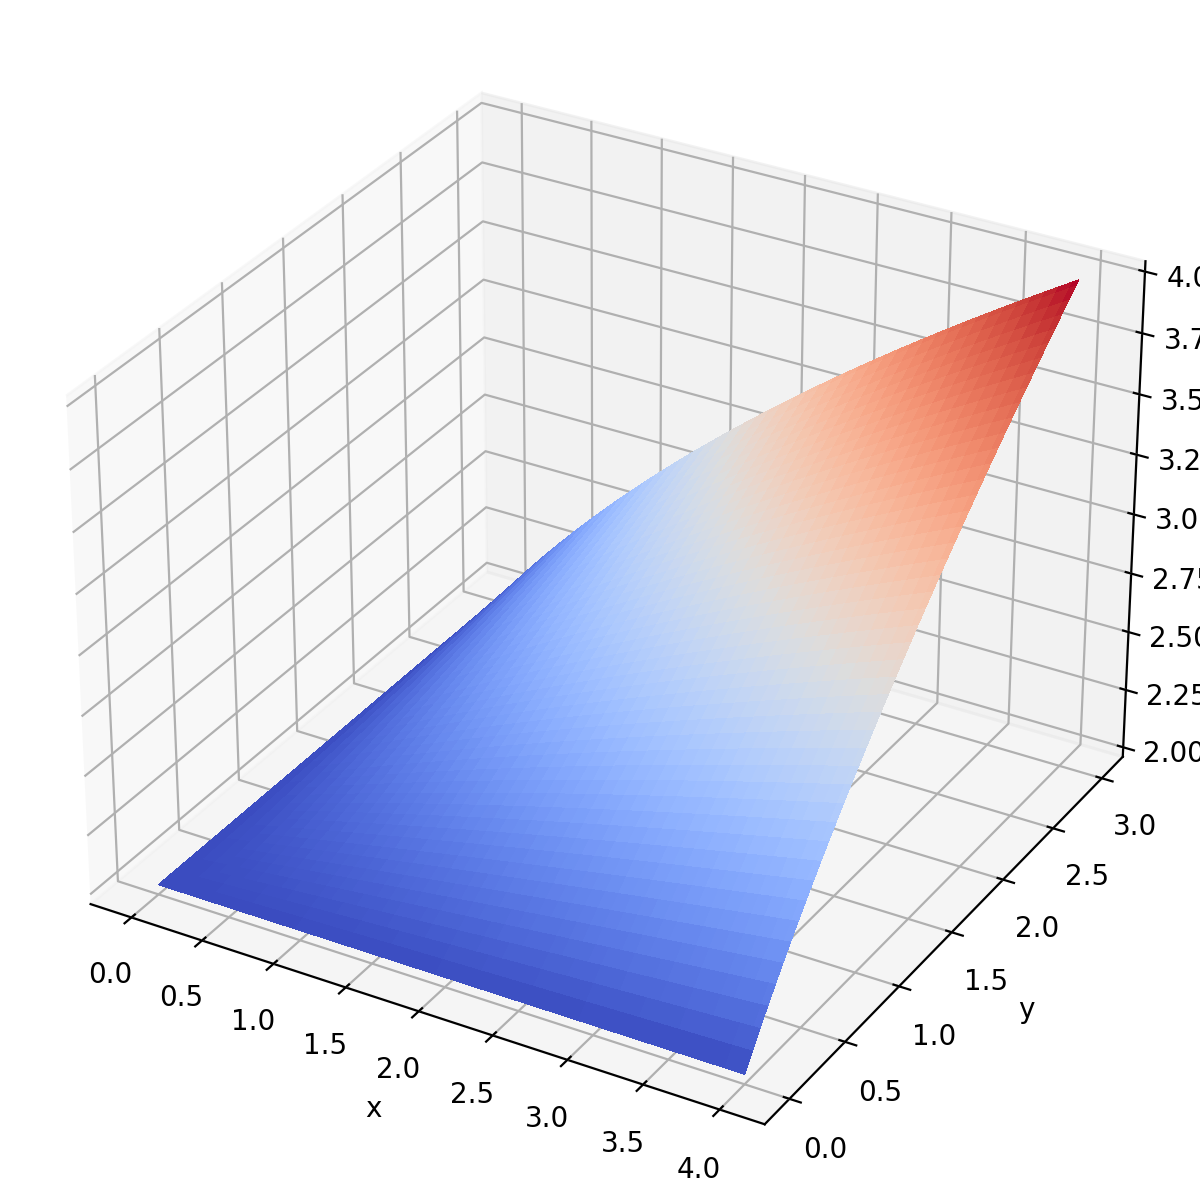
\includegraphics[width=10cm]{visualization_of_results_real.png}
    \caption{График точного решения $u(x,y) = \sqrt{4+xy}$}
    \label{fig:my_label}
\end{figure}

\begin{figure}[!htp]
    \centering
    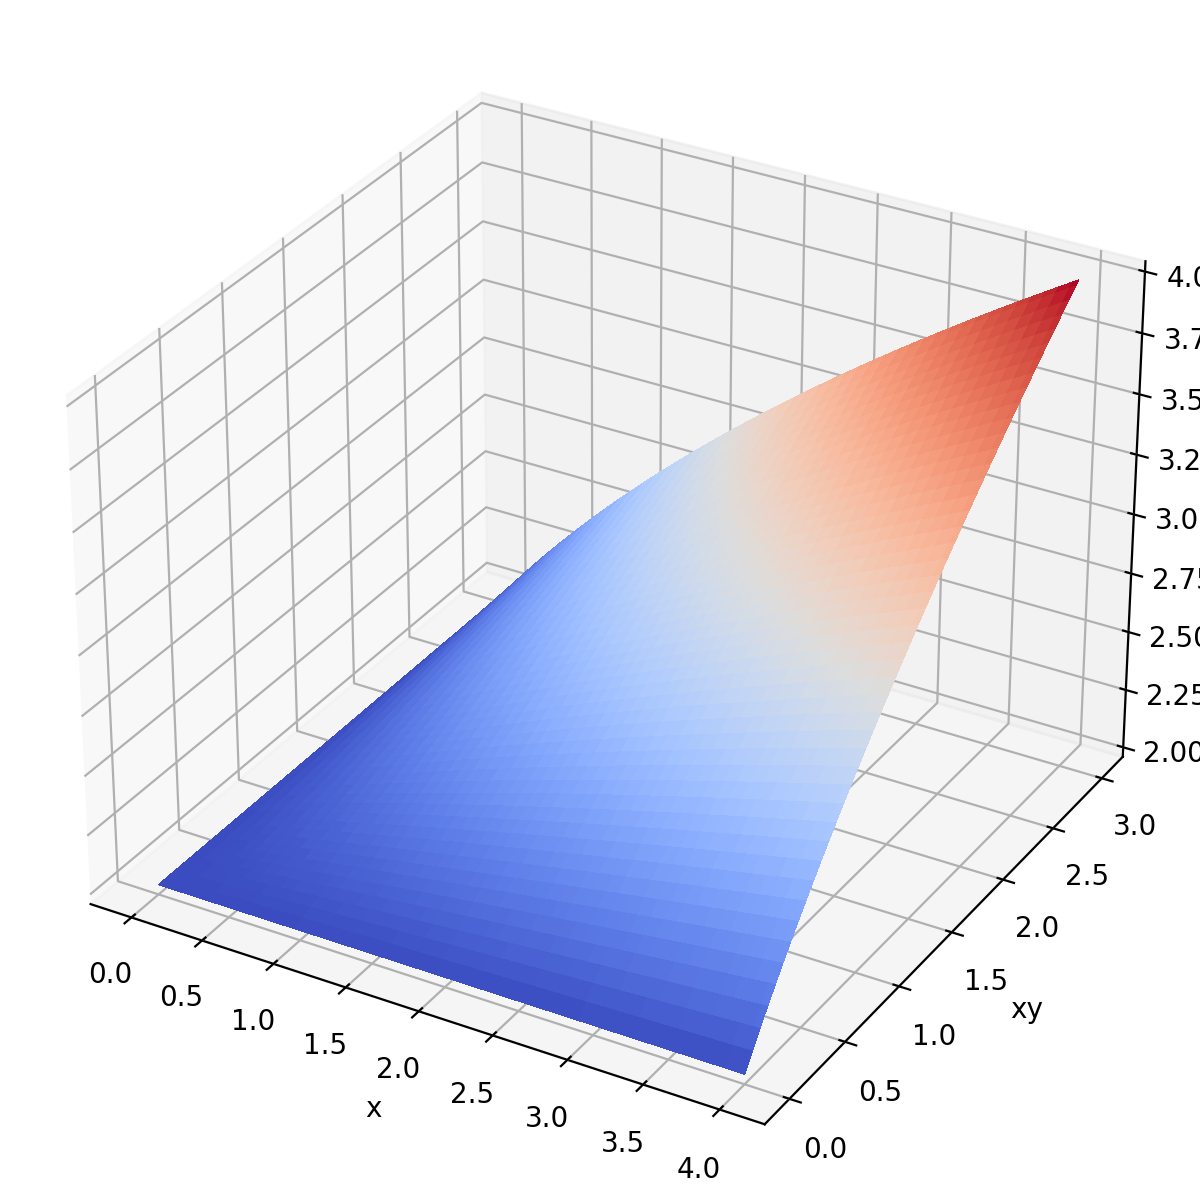
\includegraphics[width=10cm]{visualization_of_results_approx.png}
    \caption{График приближенного решения, полученного на сетке 1000 $\times$ 1000}
    \label{fig:my_label}
\end{figure}
\end{document}
